\documentclass[12pt]{article}
\usepackage{amsmath,amssymb,bookmark,parskip,tikz,custom}
\usepackage[margin=.8in]{geometry}
\allowdisplaybreaks
\hypersetup{colorlinks,
    citecolor=black,
    filecolor=black,
    linkcolor=black,
    urlcolor=black
}
\setcounter{secnumdepth}{5}

\usetikzlibrary{shapes}
\tikzstyle{bplus}=[rectangle split, rectangle split horizontal, rectangle split ignore empty parts, draw]
\tikzstyle{every node}=[bplus]
\tikzstyle{level 3}=[sibling distance=10mm]

\begin{document}

\title{CS 348 --- Assignment 2}
\author{Kevin Carruthers}
\date{\vspace{-2ex}Fall 2015}
\maketitle\HRule

\section{Question 1}
\subsection{Part A}
\subsubsection{Insert 1}
\begin{center}

\begin{tikzpicture}
\tikzstyle{level 1}=[sibling distance=30mm]
\tikzstyle{level 2}=[sibling distance=10mm]
  \node {1};
\end{tikzpicture}
\end{center}

\subsubsection{Insert 79}
\begin{center}
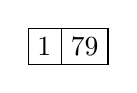
\begin{tikzpicture}
\tikzstyle{level 1}=[sibling distance=30mm]
\tikzstyle{level 2}=[sibling distance=10mm]
  \node {1 \nodepart{two} 79};
\end{tikzpicture}
\end{center}

\subsubsection{Insert 98}
\begin{center}
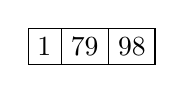
\begin{tikzpicture}
\tikzstyle{level 1}=[sibling distance=30mm]
\tikzstyle{level 2}=[sibling distance=10mm]
  \node {1 \nodepart{two} 79 \nodepart{three} 98};
\end{tikzpicture}
\end{center}

\subsubsection{Insert 4}
\begin{center}
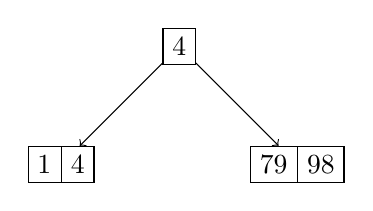
\begin{tikzpicture}
\tikzstyle{level 1}=[sibling distance=30mm]
\tikzstyle{level 2}=[sibling distance=10mm]
\node {4} [->]
  child {node {1 \nodepart{two} 4}}
  child {node {79 \nodepart{two} 98}};
\end{tikzpicture}
\end{center}

\subsubsection{Insert 69}
\begin{center}
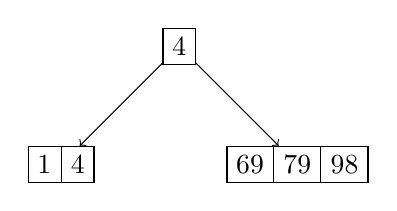
\begin{tikzpicture}
\tikzstyle{level 1}=[sibling distance=30mm]
\tikzstyle{level 2}=[sibling distance=10mm]
\node {4} [->]
  child {node {1 \nodepart{two} 4}}
  child {node {69 \nodepart{two} 79 \nodepart{three} 98}};
\end{tikzpicture}
\end{center}

\subsubsection{Insert 2}
\begin{center}
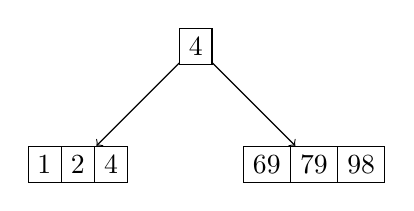
\begin{tikzpicture}
\tikzstyle{level 1}=[sibling distance=30mm]
\tikzstyle{level 2}=[sibling distance=10mm]
\node {4} [->]
  child {node {1 \nodepart{two} 2 \nodepart{three} 4}}
  child {node {69 \nodepart{two} 79 \nodepart{three} 98}};
\end{tikzpicture}
\end{center}

\subsubsection{Insert 3}
\begin{center}
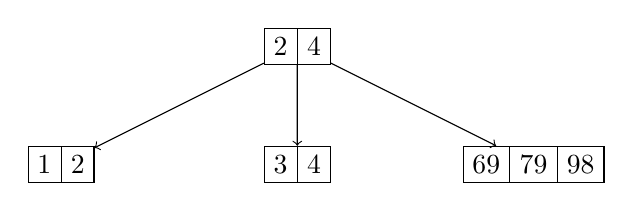
\begin{tikzpicture}
\tikzstyle{level 1}=[sibling distance=30mm]
\tikzstyle{level 2}=[sibling distance=10mm]
\node {2 \nodepart{two} 4} [->]
  child {node {1 \nodepart{two} 2}}
  child {node {3 \nodepart{two} 4}}
  child {node {69 \nodepart{two} 79 \nodepart{three} 98}};
\end{tikzpicture}
\end{center}

\subsubsection{Insert 9}
\begin{center}
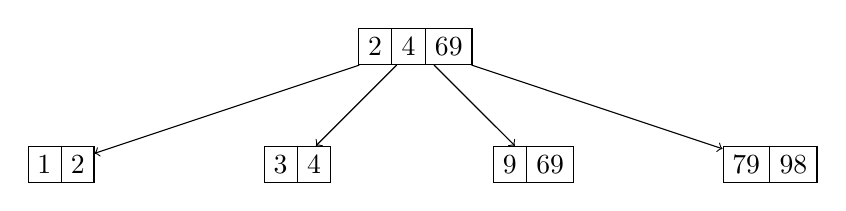
\begin{tikzpicture}
\tikzstyle{level 1}=[sibling distance=30mm]
\tikzstyle{level 2}=[sibling distance=10mm]
\node {2 \nodepart{two} 4 \nodepart{three} 69} [->]
  child {node {1 \nodepart{two} 2}}
  child {node {3 \nodepart{two} 4}}
  child {node {9 \nodepart{two} 69}}
  child {node {79 \nodepart{two} 98}};
\end{tikzpicture}
\end{center}

\subsubsection{Insert 8}
\begin{center}
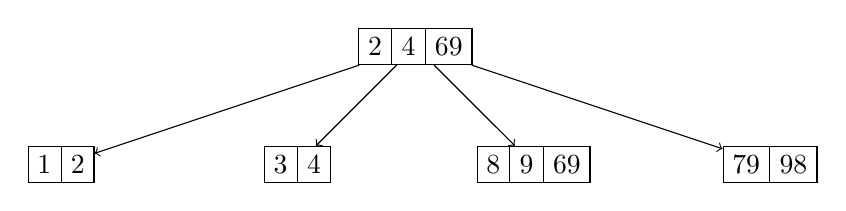
\begin{tikzpicture}
\tikzstyle{level 1}=[sibling distance=30mm]
\tikzstyle{level 2}=[sibling distance=10mm]
\node {2 \nodepart{two} 4 \nodepart{three} 69} [->]
  child {node {1 \nodepart{two} 2}}
  child {node {3 \nodepart{two} 4}}
  child {node {8 \nodepart{two} 9 \nodepart{three} 69}}
  child {node {79 \nodepart{two} 98}};
\end{tikzpicture}
\end{center}

\subsubsection{Insert 54}
\begin{center}
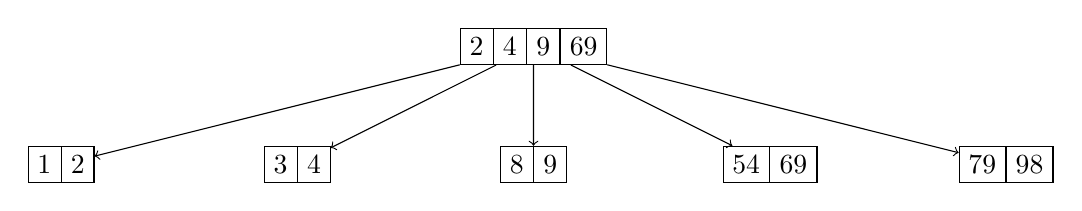
\begin{tikzpicture}
\tikzstyle{level 1}=[sibling distance=30mm]
\tikzstyle{level 2}=[sibling distance=10mm]
\node {2 \nodepart{two} 4 \nodepart{three} 9 \nodepart{four} 69} [->]
  child {node {1 \nodepart{two} 2}}
  child {node {3 \nodepart{two} 4}}
  child {node {8 \nodepart{two} 9}}
  child {node {54 \nodepart{two} 69}}
  child {node {79 \nodepart{two} 98}};
\end{tikzpicture}
\end{center}

\subsubsection{Insert 92}
\begin{center}
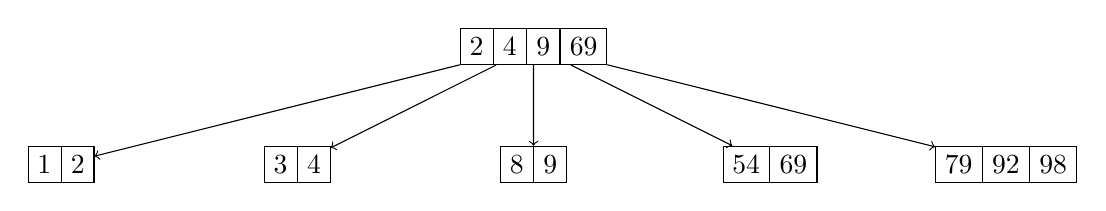
\begin{tikzpicture}
\tikzstyle{level 1}=[sibling distance=30mm]
\tikzstyle{level 2}=[sibling distance=10mm]
\node {2 \nodepart{two} 4 \nodepart{three} 9 \nodepart{four} 69} [->]
  child {node {1 \nodepart{two} 2}}
  child {node {3 \nodepart{two} 4}}
  child {node {8 \nodepart{two} 9}}
  child {node {54 \nodepart{two} 69}}
  child {node {79 \nodepart{two} 92 \nodepart{three} 98}};
\end{tikzpicture}
\end{center}

\subsubsection{Insert 97}
\begin{center}
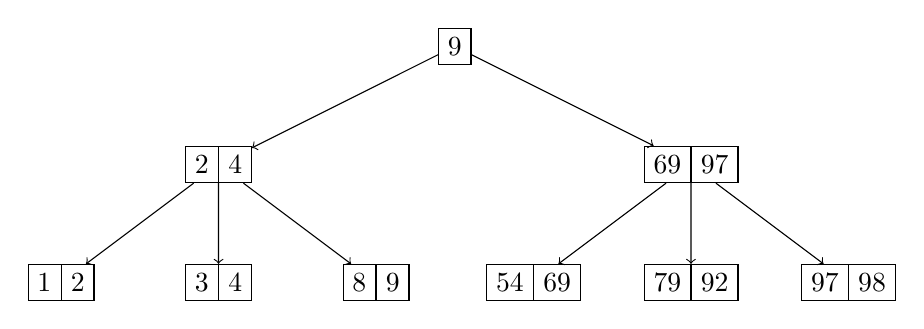
\begin{tikzpicture}
\tikzstyle{level 1}=[sibling distance=60mm]
\tikzstyle{level 2}=[sibling distance=20mm]
\node {9} [->]
  child {node {2 \nodepart{two} 4}
    child {node {1 \nodepart{two} 2}}
    child {node {3 \nodepart{two} 4}}
    child {node {8 \nodepart{two} 9}}
  }
  child {node {69 \nodepart{two} 97}
    child {node {54 \nodepart{two} 69}}
    child {node {79 \nodepart{two} 92}}
    child {node {97 \nodepart{two} 98}}
  };
\end{tikzpicture}
\end{center}

\subsection{Part B}
\subsubsection{Delete 69}
\begin{center}
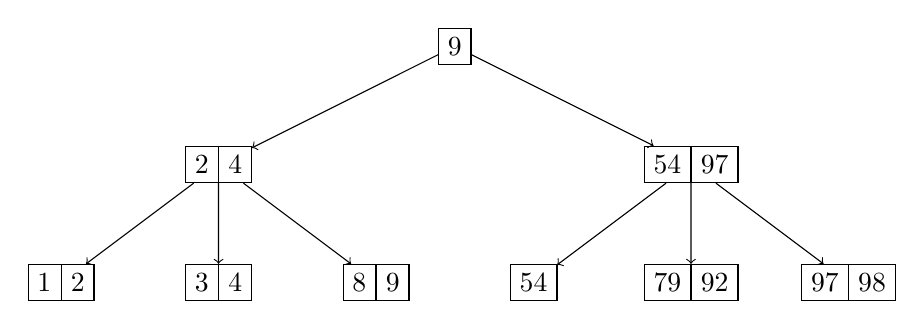
\begin{tikzpicture}
\tikzstyle{level 1}=[sibling distance=60mm]
\tikzstyle{level 2}=[sibling distance=20mm]
\node {9} [->]
  child {node {2 \nodepart{two} 4}
    child {node {1 \nodepart{two} 2}}
    child {node {3 \nodepart{two} 4}}
    child {node {8 \nodepart{two} 9}}
  }
  child {node {54 \nodepart{two} 97}
    child {node {54}}
    child {node {79 \nodepart{two} 92}}
    child {node {97 \nodepart{two} 98}}
  };
\end{tikzpicture}
\end{center}

\subsubsection{Delete 54}
\begin{center}
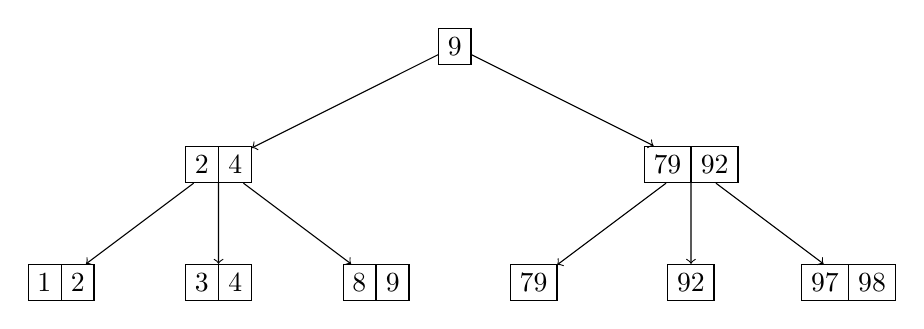
\begin{tikzpicture}
\tikzstyle{level 1}=[sibling distance=60mm]
\tikzstyle{level 2}=[sibling distance=20mm]
\node {9} [->]
  child {node {2 \nodepart{two} 4}
    child {node {1 \nodepart{two} 2}}
    child {node {3 \nodepart{two} 4}}
    child {node {8 \nodepart{two} 9}}
  }
  child {node {79 \nodepart{two} 92}
    child {node {79}}
    child {node {92}}
    child {node {97 \nodepart{two} 98}}
  };
\end{tikzpicture}
\end{center}

\subsubsection{Delete 92}
\begin{center}
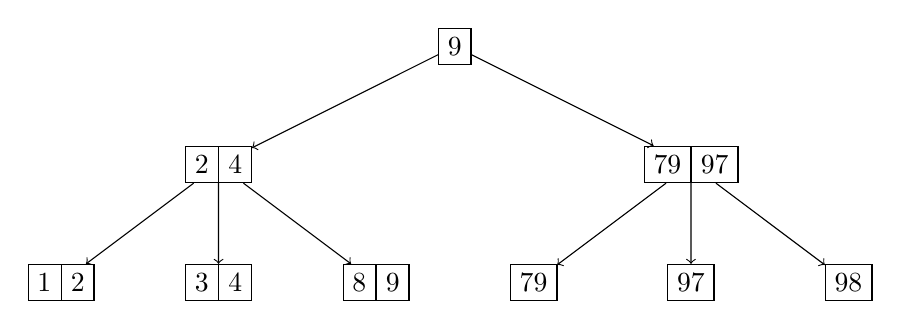
\begin{tikzpicture}
\tikzstyle{level 1}=[sibling distance=60mm]
\tikzstyle{level 2}=[sibling distance=20mm]
\node {9} [->]
  child {node {2 \nodepart{two} 4}
    child {node {1 \nodepart{two} 2}}
    child {node {3 \nodepart{two} 4}}
    child {node {8 \nodepart{two} 9}}
  }
  child {node {79 \nodepart{two} 97}
    child {node {79}}
    child {node {97}}
    child {node {98}}
  };
\end{tikzpicture}
\end{center}

\subsubsection{Delete 97}
\begin{center}
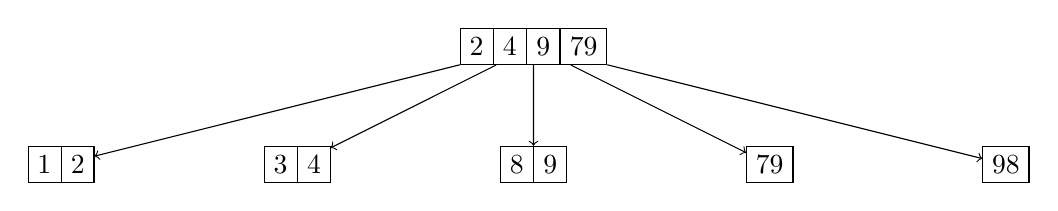
\begin{tikzpicture}
\tikzstyle{level 1}=[sibling distance=30mm]
\tikzstyle{level 2}=[sibling distance=10mm]
\node {2 \nodepart{two} 4 \nodepart{three} 9 \nodepart{four} 79} [->]
  child {node {1 \nodepart{two} 2}}
  child {node {3 \nodepart{two} 4}}
  child {node {8 \nodepart{two} 9}}
  child {node {79}}
  child {node {98}}
;
\end{tikzpicture}
\end{center}

\section{Question 2}
\begin{figure}[ht]
\centering
\includegraphics[width=0.8\textwidth]{a2schema.png}
\end{figure}

\end{document}
